\section{ОБЗОР МЕТОДОВ И СИСТЕМ \\ОБНАРУЖЕНИЯ КОМПЬЮТЕРНЫХ АТАК}

В данном разделе приведен обзор основных методов обнаружения компьютерных атак, используемых в современных СОА, а также нескольких некоммерческих СОА.
Целью обзора является исследовать эффективность доступных в настоящее время СОА и определить основные недостатки используемых в них методов обнаружения атак. Основная сложность составления подобного обзора заключается в том, что множество доступных реализаций СОА представлено, в основном, коммерческими системами (такими как Cisco IPS, Juniper NetScreen, ISS RealSecure, NFR и т.д.), для которых отсутствует открытая информация о программной архитектуре и используемым формальным методам обнаружения атак. Доступная информация по подобным системам носит маркетинговый характер, что затрудняет проведение сравнительного анализа по публикациям в литературе. По этой причине множество рассматриваемых в обзоре систем будет ограничено СОА с открытым исходным кодом, доступным публично.
В результате обзора будет показано, что:

\begin{enumerate}

\item Большинство современных СОА используют на базовом уровне ту или иную реализацию сигнатурного метода обнаружения (pattern matching, сравнение шаблонов). Реализации отличаются друг от друга уровнем рассмотрения системы, алфавитом сигнатур и используемым <<движком>> --- от простого поиска подстрок до полноценной реализации регулярных выражений над заданным алфавитом.
\item Множество существующих методов обнаружения атак много шире, но их использование в системах имеет принципиальные ограничения, связанные с требованиями верифицируемости, устойчивости и воспроизводимости результата, а также большим числом ошибок второго рода (ложных срабатываний). Использование таких методов ограничено экспериментальными академическими разработками.
\item Доступные реализации СОА неустойчивы к модификациям атак и не могут автоматически адаптироваться к появлению новых атак. При этом использование методов обнаружения аномалий (например, в препроцессорах СОА Snort) ограничено по причинам, перечисленным в п.2.

\end{enumerate}


% \textbf{Штрихкод} (сокр. от << код}>>, англ. 
% <<\textit{bar code}>>) --- графическая информация наносимая на 
% поверхности предметов, предназначенная для обработки техническими
% средствами.

% Выделяют две большие группы штрихкодов: \textit{линейные} 
% и \textit{двухмерные}.
% В первом случае информационную нагрузку имеют только чередования 
% участков различной яркости по одной из осей, во втором --- по обеим.


\subsection{\textsc{Критерии сравнения}}  

В обзоре используются две группы критериев: первая группа характеризует собственно методы обнаружения атак и специфичные для них качественные и количественные показатели эффективности, в то время как вторая группа критериев характеризует реализации этих методов в системах обнаружения атак.

\subsubsection{Критерии сравнения методов обнаружения атак}

Для сравнительного анализа методов обнаружения атак выбраны следующие критерии:

\textbf{Уровень наблюдения за системой:} Данный критерий определяет уровень абстракции анализируемых событий в защищаемой системе и определяет границы применимости метода для обнаружения атак в сетях. В рамках данного обзора рассматриваются следующие уровни:

\begin{itemize}

\item HIDS --- наблюдение на уровне операционной системы отдельного узла сети
\item NIDS --- наблюдение на уровне сетевого взаимодействия объектов на узлах сети
\item AIDS --- наблюдение на уровне отдельных приложений узла сети
\item Hybrid --- комбинация наблюдателей разных уровней

\end{itemize}

\textbf{Верифицируемость метода:} Данный критерий позволяет оценить, может ли человек (например, квалифицированный оператор СОА или эксперт) воспроизвести последовательность шагов по принятию решения о наличии атаки, сопоставляя входные и выходные данные СОА. Например, сигнатурные методы будем считать верифицируемыми, а кластерные – нет. Верифицируемость позволяет провести экспертную оценку корректности метода и его реализации в произвольный момент времени, в том числе в процессе эксплуатации системы обнаружения на его основе. Свойство верифицируемости метода важно при эксплуатации системы обнаружения атак в реальной обстановке в качестве средства сбора доказательной базы об атаках.

Возможные значения: высокая (+), низкая (-).

\textbf{Адаптивность метода:} Оценка устойчивости метода к малым изменениям реализации атаки, которые не изменяют результат атаки. Адаптивность является единственным существенным преимуществом <<альтернативных>> методов обнаружения атак перед <<сигнатурными>>. Отсутствие адаптивности не позволяет системе защиты оперативно реагировать на неизвестные атаки и требует организации системы регулярного обновления баз известных атак, по аналогии с антивирусными системами. Возможные значения: высокая (+), низкая (-).

\textbf{Устойчивость:} Данный критерий характеризует независимость выхода метода от защищаемой системы --- для одного и того же входа метод должен давать один и тот же выход, независимо от защищаемой системы. Проблема устойчивости особенно остро стоит для статистических методов, анализирующих абсолютные значения параметров производительности и загруженности ресурсов сети и узлов, которые могут существенно отличаться на различных узлах и в различных сетях. Обученный в одной сети распознаватель может быть устойчивым в пределах данной сети и неустойчивым во всех остальных сетях. Такую устойчивость будем называть локальной. Так как процедура обучения обычно является <<дорогой>> --- требует использования большого количества ресурсов и времени --- число процедур обучения желательно минимизировать. Методы обнаружения атак, анализирующие семантику ввода, более устойчивы, чем статистические. Возможные значения: глобальная (+), локальная (-).


\textbf{Вычислительная сложность:} Теоретическая оценка сложности метода на основе информации из публикаций. В обзоре рассматривается только сложность метода в режиме обнаружения, без учёта возможных предварительных этапов настройки и обучения. Данный критерий является ключевым для задачи обнаружения атак в сетях и имеет гораздо большее значение, нежели сложность по памяти из-за опережающего роста пропускной способности каналов передачи данных и удешевления машинной памяти.

\begin{itemize}

\item Сублинейная --- константа, логарифм

\item Линейная

\item Квадратичная и т.д.

\end{itemize}

В обзоре не рассмотрены такие важные критерии как полнота и точность метода, т.к. эти характеристики редко приводятся в публикациях.

\subsubsection{Критерии сравнения систем обнаружения атак}

Для сравнительного анализа СОА были выбраны следующие критерии:\\
\textbf{Класс обнаруживаемых атак.} Данный критерий определяет, какие классы атак способна обнаружить рассматриваемая система. Это один из ключевых критериев. В связи с тем, что на сегодняшний день ни одна система не способна обнаружить атаки всех классов, для более полного покрытия всего спектра атак необходимо комбинировать различные СОА. Здесь мы используем классификацию атак, основанную на разделении ресурсов защищаемой системы по типам.

Класс атаки – это четверка <\textbf{L,R,A,D}>, где L --- расположение атакующего объекта, R --- атакуемый ресурс, A --- целевое воздействие на ресурс, D --- признак распределенного характера атаки.

\textbf{L:} расположение атакующего объекта. Оно может быть либо внутренним по отношению к защищаемой системе \textbf{(li)}, либо внешним \textbf{(le)}.

\textbf{R:} атакуемый ресурс. Ресурсы разделяются по расположению и по типу.

\begin{itemize}

\item По расположению: узловые \textbf{(rl)}, сетевые \textbf{(rn)}.

\item По типу: пользовательские ресурсы \textbf{(ru)}, системные ресурсы \textbf{(rs)}, ресурсы СУБД \textbf{(rd)}, вычислительные ресурсы \textbf{(rc)}, ресурсы защиты \textbf{(rp)}.

\end{itemize}

\textbf{A:} целевое воздействие на ресурс: сбор информации \textbf{(as)}, получение прав пользователя ресурса \textbf{(au)}, получение прав администратора ресурса \textbf{(ar)}, нарушение целостности ресурса \textbf{(ai)}, нарушение работоспособности ресурса \textbf{(ad)}.

\textbf{D:} признак распределенного характера атаки: распределенные \textbf{(dd)}, нераспределенные \textbf{(dn)}.

Следующий критерий характеризует источники и способы сбора информации о поведении объектов и состоянии ресурсов:\\

\textbf{Уровень наблюдения за системой.} Определяет, на каком уровне защищаемой системы собирают данные для обнаружения атаки. Различаются узловые и сетевые источники. В пределах узловых источников разделяются уровни ядра и приложения. От уровня наблюдения за системой зависит скорость сбора информации, влияние системы на собираемую информацию, вероятность получения искаженной информации. Следует отметить, что использование метода обнаружения, позволяющего анализировать поведение на всех уровнях абстракции, не означает, что эта возможность реализована в конкретной системе. Зачастую реализация обладает меньшими возможностями, чем теоретические возможности используемого ею метода. 

\begin{itemize}

\item HIDS --- наблюдение на уровне операционной системы отдельного узла сети
\item NIDS --- наблюдение на уровне сетевого взаимодействия объектов на узлах сети
\item AIDS --- наблюдение на уровне отдельных приложений узла сети
\item Hybrid --- комбинация наблюдателей разных уровней

\end{itemize}

Следующий критерий определяет эффективность обнаружения атаки на основе анализа полученной информации.
\textbf{Используемый метод обнаружения.} Метод обнаружения также является ключевым критерием сравнения. Существует два класса методов: \textit{методы обнаружения аномалий} и \textit{методы обнаружения злоупотреблений}. В приведенном ниже списке перечислены не отдельные методы, но, в основном, семейства методов, объединённых некоторым единым подходом или теоретической моделью. 
\begin{itemize}

\item Обнаружение злоупотреблений

\begin{itemize}

\item Анализ систем состояний
\item Графы атак
\item Нейронные сети
\item Иммунные сети
\item SVM
\item Экспертные системы
\item Методы, основанные на спецификациях
\item MARS – Multivariate Аdaptive Regression Splines
\item Сигнатурные методы

\end{itemize}

\item Обнаружение аномалий

\begin{itemize}

\item Статистический анализ
\item Кластерный анализ (data mining)
\item Нейронные сети
\item Иммунные сети
\item Экспертные системы
\item Поведенческая биометрия
\item SVM
\item Анализ систем состояний

\end{itemize}

\end{itemize} 

\textbf{Адаптивность к неизвестным атакам.} Определяет способность используемого
метода обнаруживать ранее неизвестные атаки.\\
Следующие критерии определяют такие архитектурные особенности СОА как управление и распределенность.

\textbf{Масштабируемость.} Определяет возможность добавления новых анализируемых ресурсов сети, новых узлов и каналов передачи данных, в том числе возможность управления единой распределенной системой обнаружения атак. Управление может быть централизованное и/или распределенное. Дополнительно может присутствовать возможность удаленного управления СОА. Сюда включаются задачи установки, настройки и администрирования системы. При полностью распределенном управлении необходимо управлять всеми компонентами СОА в отдельности. При полностью централизованном управлении все компоненты СОА могут управляться с одного узла. Оптимальной представляется организация управления по централизованной схеме, в которой может быть несколько центров, и они могут динамически меняться.

\textbf{Открытость.} Определяет насколько система является открытой для интеграции в нее других методов обнаружения атак, компонентов сторонних разработчиков и сопряжения ее с другими системами защиты информации. Это могут быть программные интерфейсы для встраивания дополнительных модулей и/или реализация стандартов взаимодействия сетевых компонентов.

\textbf{Формирование ответной реакции на атаку.} Определяет наличие в системе встроенных механизмов ответной реакции на атаку, кроме самого факта ее регистрации. Примерами реакции могут быть разрыв соединения с атакующим объектом, блокировка его на межсетевом экране, отслеживание пути проникновения атакующего объекта в защищаемую систему и т.д.

\textbf{Защищенность.} Определяет степень защищенности СОА от атак на ее компоненты, включая защиту передаваемой информации, устойчивость к частичному выходу компонентов из строя или их компрометации. Затрагиваются такие вопросы, как наличие уязвимостей в компонентах СОА, защищенность каналов передачи данных между ними, а также авторизация компонентов внутри СОА.

Таким образом, некая <<идеальная>> система обнаружения атак обладает следующими свойствами:
\begin{itemize}

\item покрывает все классы атак (система полна)
\item позволяет анализировать поведение защищаемой РИС на всех уровнях: сетевом, узловом и уровне отдельных приложений
\item адаптивна к неизвестным атакам (использует адаптивный метод обнаружения атак)
\item масштабируется для РИС различных классов: от небольших локальных сетей класса <<домашний офис>> до крупных многосегментных и коммутированных корпоративных сетей, обеспечивая возможность централизованного управления всеми компонентами СОА
\item является открытой
\item имеет встроенные механизмы реагирования на атаки
\item является защищённой от атак на компоненты СОА, в том числе от перехвата управления или атаки <<отказ в обслуживании>>.

\end{itemize}

\subsection{\textsc{Методы обнаружения атак}}

Все методы обнаружения атак можно разделить на два класса: методы обнаружения аномалий и методы обнаружения злоупотреблений. Методы первого класса базируются на наличии готового описания нормального поведения наблюдаемых объектов РИС, и любое отклонение от нормального поведения считается аномальным (нарушением). Методы обнаружения злоупотреблений основаны на описании известных нарушений или атак: если наблюдаемое поведение некоторого объекта РИС совпадает с описанием известной атаки, поведение объекта считается атакой.

\subsubsection{Методы обнаружения злоупотреблений}

\textbf{Анализ систем состояний:} В данной группе методов функционирование защищаемой системы представляется через множество состояний и множество переходов между ними, т.е. в виде ориентированного графа (как правило, бесконечного). Суть метода обнаружения атак заключается в том, что часть путей в таком графе помечаются как недопустимые; конечное состояние каждого такого пути считается опасным для защищаемой системы. Процесс обнаружения атаки представляет собой построение части графа состояний системы и наблюдаемых переходов между ними, и поиск в полученном графе известных недопустимых путей. Обнаружение последовательности переходов, приводящей в опасное состояние, означает успешное обнаружение атаки. В соответствии с введёнными критериями, данный метод является гибридным с точки зрения уровня наблюдения за системой, верифицируемым, устойчивым, имеет низкую вычислительную сложность (линейную относительно длины трассы наблюдаемых переходов и числа состояний), но не является адаптивным.

\textbf{Графы сценариев атак:} На вход системе верификации подаётся конечная модель защищаемой системы и некоторое формальное свойство корректности, которое выполняется только для разрешённого поведения системы. Данное свойство корректности делит всё множество поведений на два класса --- допустимого поведения, для которого свойство выполняется, и недопустимого, для которого оно не выполняется. Отличие данного метода от обычных систем верификации заключается в том, что их задача, обычно, найти один контрпример из множества недопустимого поведения, а в предложенном методе строится полный набор таких примеров для конкретной защищаемой системы, что даёт на выходе описание возможных путей атаки. Из-за высокой вычислительной сложности (NP) данный метод может быть использован для поиска уязвимостей проектирования систем и других сложных для обнаружения уязвимостей, но для задачи обнаружения атак в реальном времени он неприменим. По остальным критериям метод является гибридным, верифицируемым, устойчивым и адаптивным.

\textbf{Нейронные сети:} Так как задачу обнаружения атак можно рассматривать как задачу распознавания образов (или задачу классификации), то для её решения также применяются нейронные сети. Для этого функционирование защищаемой системы и взаимодействующих с ней внешних объектов представляется в виде траекторий в некотором числовом пространстве признаков. В качестве метода обнаружения злоупотреблений, нейронные сети обучаются на примерах атак каждого класса и, в дальнейшем, используются для распознавания принадлежности наблюдаемого поведения одному из классов атак. Основная сложность в использовании нейросетей заключается в корректном построении такого пространства признаков, которое позволило бы разделить классы атак между собой и отделить их от нормального поведения. Кроме того, для классических нейронных сетей характерно долгое обучение, при этом время обучения зависит от размера обучающей выборки. В соответствии с введёнными критериями, нейронные сети используются на сетевом и узловом уровнях, являются адаптивными, имеют сравнительно низкую вычислительную сложность. При этом они не являются верифицируемыми и устойчивы, как правило, только в пределах той сети, в которой они обучались, что существенно ограничивает применимость метода (только локальная устойчивость).

\textbf{Иммунные сети:} Также как и нейронные сети, иммунные сети являются механизмом классификации и строятся по аналогии с иммунной системой живого организма. Основное достоинство иммунных сетей заключатся в возможности получения <<антител>> к неизвестным атакам. В одной работе (РАБОТА) была предложена модель формального пептида, для которой заявлена возможность использования в системах обнаружения атак. Однако, позже было показано, что использование данного метода требует решения системы дифференциальных уравнений в режиме обнаружения, что даёт вычислительную сложность порядка $O(n^3)$ при использовании метода Рунге-Кутта. В соответствии с введёнными критериями, данная группа методов применима для сетевого и узлового уровней, не верифицируема, адаптивна, устойчива только локально, имеет высокую вычислительную сложность.

\textbf{Support vector machines (SVM):} SVM – это метод представления и распознания шаблонов, который позволяет формировать шаблоны в результате обучения. Данный метод требует небольшого количества данных для обучения и позволяет обрабатывать векторы признаков большой размерности, что полезно для повышения точности систем обнаружения атак и снижения временных затрат на обучение и переобучение. Метод применим как для обнаружения злоупотреблений, так и для обнаружения аномалий. SVM имеет такие же достоинства и недостатки для решения нашей задачи, как и нейронные сети, т.е. является адаптивным, но неверифицируемым.

\textbf{Экспертные системы:} Использование экспертных систем для обнаружения атак основано на описании функционирования системы в виде множества фактов и правил вывода, в том числе для атак. На вход экспертная система получает данные о наблюдаемых событиях в системе в виде фактов. На основании фактов и правил вывода система делает вывод о наличии или отсутствии атаки. Данная группа методов удовлетворяет практически всем критериям (верифицируема, адаптивна, устойчива), но в общем случае имеет очень большую вычислительную сложность, так как для нее может наблюдаться явление <<комбинаторного взрыва>> и полного перебора большого числа альтернатив.

\textbf{Методы, основанные на спецификациях:} В основе данного метода лежит описание ограничений на запрещенное поведение объектов в защищаемой системе в виде спецификаций атак. В спецификацию может входить: ограничения на загрузку ресурсов, на список запрещенных операций и их последовательностей, на время суток, в течение которого применимы те или иные ограничения. Соответствие поведения спецификации считается атакой. Спецификации используются для сетевого уровня, является верифицируемым, локально устойчивым и имеет низкую вычислительную сложность. Данный подход близок к классу методов обнаружения аномалий. Основные недостатки --- низкая адаптивность и сложность разработки спецификаций.

\textbf{Multivariate Adaptive Regression Splines (MARS):} Один из методов аппроксимации функций, основанный на сплайнах. Аналогично нейронным сетям и кластерному анализу MARS оперирует в многомерном пространстве признаков. Поведение сетевых объектов отображается в последовательности векторов данного пространства. Задача процедуры MARS заключается в построении оптимальной аппроксимации поведения по заданной истории в виде обучающего множества векторов, при этом в качестве аппроксимирующей функции используются сплайны с переменным числом вершин. В ходе <<обучения>>, с помощью переборного процесса, выбирается оптимальное число вершин для заданной выборки. Построенный сплайн является <<шаблоном>> атаки. В режиме распознавания наблюдаемое поведение отображается в параметрическое пространство и сравнивается с аппроксимирующей функцией. Достоинства и недостатки данного метода аналогичны SVM и нейронным сетям.

\textbf{Сигнатурные методы:} Наиболее часто используемая группа методов, суть которых заключается в составлении некоторого алфавита из наблюдаемых в системе событий и описании множества сигнатур атак в виде регулярных выражений (в общем случае) в построенном алфавите. Как правило, сигнатурные методы работают на самом низком уровне абстракции и анализируют непосредственно передаваемые по сети данные, параметры системных вызовов и записи файлов журналов. В наиболее развитом виде представляет собой реализацию регулярных выражений над различными трассами (сетевой трафик, системные вызовы, записи журналов приложений и т.п.). Сигнатурные методы примечательны тем, что для них хорошо применимы аппаратные ускорители, но при этом метод не является адаптивным. По остальным критериям данная группа методов является гибридной, глобально устойчивой, верифицируемой. 

\subsubsection{Методы обнаружения аномалий}

\textbf{Статистический анализ:} Данная группа методов основана на построении статистического профиля поведения системы в течение некоторого периода <<обучения>>, при котором поведение системы считается нормальным [4,87]. Для каждого параметра функционирования системы строится интервал допустимых значений, с использованием некоторого известного закона распределения. Далее, в режиме обнаружения, система оценивает отклонения наблюдаемых значений от значений, полученных во время обучения. Если отклонения превышают некоторые заданные значения, то фиксируется факт аномалии (атаки). Для статистического анализа характерен высокий уровень ложных срабатываний при использовании в локальных сетях, где поведение объектов не имеет гладкого, усреднённого характера. Кроме того, данный метод устойчив только в пределах конкретной системы, то есть построенные статистические профили нельзя использовать на других аналогичных системах. 

\textbf{Кластерный анализ:} Суть данной группы методов состоит в разбиении множества наблюдаемых векторов-свойств системы на кластеры, среди которых выделяют кластеры нормального поведения. В каждом конкретном методе кластерного анализа используется своя метрика, которая позволяет оценивать принадлежность наблюдаемого вектора свойств системы одному из кластеров или выход за границы известных кластеров. Кластерный анализ является адаптивным, но не верифицируемым и устойчивым в пределах конкретной системы, в которой собирались данные для построения кластеров.

\textbf{Нейронные сети:} Нейронные сети для обнаружения аномалий обучаются в течение некоторого периода времени, когда всё наблюдаемое поведение считается нормальным. После обучения нейронная сеть запускается в режиме распознавания. В ситуации, когда во входном потоке не удается распознать нормальное поведение, фиксируется факт атаки. В случае использования репрезентативной обучающей выборки нейронные сети дают хорошую устойчивость в пределах заданной системы; но составление подобной выборки является серьёзной и сложной задачей.  Классические нейронные сети имеют высокую вычислительную сложность обучения, что затрудняет их применение на больших потоках данных. 

\textbf{Иммунные сети:} Обнаружение аномалий является одним из возможных приложений иммунных методов. Так как количество примеров нормального поведения обычно на порядки превышает число примеров атак, использование иммунных сетей для обнаружения анормалий имеет большую вычислительную сложность. 

\textbf{Экспертные системы:} Информация о нормальном поведении представляется в подобных системах в виде правил, а наблюдаемое поведение в виде фактов. На основании фактов и правил принимается решение о соответствии наблюдаемого поведения<<«нормальному>>, либо о наличии аномалии. Главный недостаток подобных систем --- высокая вычислительная сложность (в общем случае). В том числе при обнаружении аномалий. 

\textbf{Поведенческая биометрия:} Включает в себя методы, не требующие специального оборудования (сканеров сетчатки, отпечатков пальцев), т.е. методы обнаружения атак, основанные на наблюдения клавиатурного почерка и использования мыши. В основе методов лежит гипотеза о различии «почерка» работы с интерфейсами ввода-вывода для различных пользователей. На базе построенного профиля нормального поведения для данного пользователя обнаруживаются отклонения от этого профиля, вызванные попытками других лиц работать с клавиатурой или другими физическими устройствами ввода. Поведенческая биометрия имеет строго локальную устойчивость (в пределах одной сети) и слабо верифицируема.

\textbf{Support vector machines (SVM):} SVM применим как для обнаружения злоупотреблений, так и для обнаружения аномалий, при этом метод имеет достоинства и недостатки, аналогичные нейронным сетям

\newcommand{\specialcell}[2][c]{%
  \begin{tabular}[#1]{@{}c@{}}#2\end{tabular}}

\subsubsection{Результаты сравнительного анализа}

{\footnotesize
\begin{center}
\begin{tabular}{ | l | c | c | c | c | c | c |}
	\hline
  \specialcell{      Критерий\\Метод} & \specialcell{Уровень\\наблюдения} & \specialcell{Аномалии / \\Злоупотр.} & Вериф & Адапт & Устойч & Выч. сложность \\ \hline
  Системы переходов & Hybrid & -/+ & + & - & + & $O(n)$ \\ \hline
  Графы атак & Hybrid & -/+ & + & + & + & $NP$ \\ \hline
  Нейронные сети & NIDS, HIDS & +/+ & - & + & - & $O(n)$ и выше \\ \hline
  Имунные сети & NIDS, HIDS & +/+ & - & + & - & $O(n)$ и выше \\ \hline
  SVM & NIDS, HIDS & +/+ & - & + & - & $ln(n)$\\ \hline
  Экспертные системы & NIDS, HIDS & +/+ & + & + & + & \specialcell{В общем случае\\$NP$}\\ \hline 
  Спецификации & NIDS & -/+ & + & - & - & $ln(n)$\\ \hline
  MARS & NIDS, HIDS & -/+ & - & + & - & $O(n)$ и выше \\ \hline
  Сигнатурные методы & Hybrid & -/+ & + & - & + & $ln(n)$ \\ \hline
  Статистические методы & NIDS, HIDS & +/- & - & + & - & $O(n)$ и выше \\ \hline
  Кластерный анализ & Hybrid & +/+ & - & + & - & $O(n)$ и выше \\ \hline
  Поведенческая биометрия & HIDS & +/- & - & + & - & $O(n)$ и выше \\ \hline
\end{tabular}\\
\textit{Таблица 1.} Результаты сравнения методов обнаружения атак.
\end{center} 
}

Таким образом, анализ публикаций показывает, что для большинства методов обнаружения аномалий характерна слабая верифицируемость и слабая глобальная устойчивость (либо её отсутствие). Основное достоинство методов обнаружения аномалий заключается в их адаптивности и способности обнаруживать ранее неизвестные атаки. Среди глобально устойчивых и верифицируемых методов, имеющих при этом низкую вычислительную сложность, можно отметить метод анализа системы переходов и простой сигнатурный метод. Ни один из рассмотренных методов не обладает одновременно адаптивностью, устойчивостью и верифицируемостью, имея при этом приемлемую вычислительную сложность.

\subsection{\textsc{Современные открытые системы обнаружения атак}}

В данном разделе рассмотрены доступные на сегодняшний день системы
обнаружения атак с открытым исходным кодом.

\subsubsection{Исследованные системы обнаружения атак}

Всего рассмотрено 5 систем обнаружения атак. В табл. 2. приведена краткая информация по каждой из них.

\begin{center}
\begin{tabular}{ | l | l | l | }

\hline
Название & Производитель & Ссылки \\ \hline
Bro & \specialcell{University of California, Lawrence\\Berkeley National Laboratory} & http://bro-ids.org/ \\ \hline
OSSEC & Daniel B. Sid, OSSEC.net & http://www.ossec.net/ \\ \hline
STAT & \specialcell{University of California\\at Santa Barbara} & http://www.cs.ucsb.edu/seclab/index.html \\ \hline
Prelude & \specialcell{Yoann Vandoorselaere,\\Laurent Oudot} & http://www.prelude-ids.org/ \\ \hline
Snort & Martin Roesch & http://www.snort.org/ \\ \hline

\end{tabular}
\end{center}


Исторически, линейные штрихкоды появились первыми (50--70-ые годы 
XX века). Коды этой группы не отличаются особым разнообразием ---
чередование чёрных и белых полос, кодирующие цифры либо буквы. Вместе
с тем, линейные коды наносятся практически на все товары 
(\figurename\ \ref{fig:ean}), 
распространяемые в розницу (формат EAN --- European Article Number),
и потому наиболее широко распространены. Другие примеры рисунки 
\ref{fig:code128}, \ref{fig:itf14}. 

В этой работе мы не будем рассматривать линейные штрихкоды.

\begin{figure}[h]
    \begin{multicols}{2}
 
        \begin{center}
             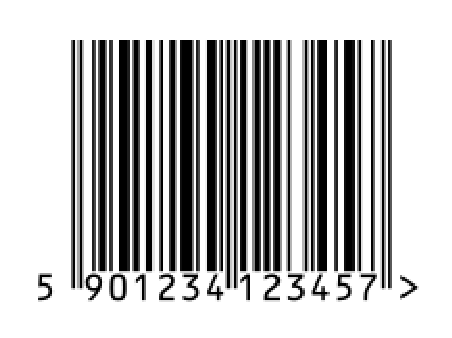
\includegraphics[scale=0.5]{img/ean_sample} 
             \caption{Штрихкод в формате EAN}
             \label{fig:ean}
        \end{center}
   
        \begin{center}
            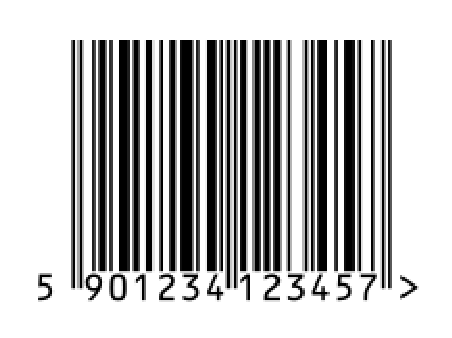
\includegraphics[scale=0.5]{img/ean_sample} 
            \caption{Штрихкод в формате Code 128}
            \label{fig:code128}
        \end{center}       
       
    \end{multicols}
\end{figure}

\begin{figure}[h]
    \centering
    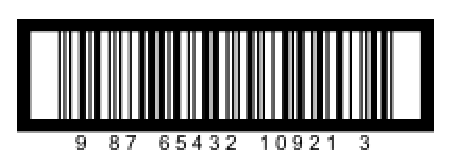
\includegraphics[scale=0.7]{img/itf_sample}
    \caption{Штрихкод в формате ITF-14}
    \label{fig:itf14}
\end{figure}
    
\subsection{\textsc{Двумерные штрихкоды}}

Как уже отмечалось, в двумерных штрихкодах информация кодируется
по обеим осям. Выделяются два вида двумерных кодов: \textit{стековые}
и \textit{матричные}.

\subsubsection{Стековые штрихкоды}  
Стековые штрикоды являются, в некоторой мере, переходным вариантом
между линейными и двухмерными. Они представляю собой строки расположенные
одна под одной. Каждая строка есть ни что иное, как одномерный штрихкод.

Несмотря на свою простоту, данный тип штрихкодов позволяет хранить 
значительные объёмы данных. Например, штрикод формата PDF417 
(см. \figurename\ \ref{fig:pdf417}) может содержать до 2710 знаков.
Стековые штрихкоды также не является объектом рассмотрения данной
работы. 

\begin{figure}[htb]
    \centering
    
\includegraphics{img/pdf417_sample}
    \caption{Штрихкод в формате PDF417}
    \label{fig:pdf417}
\end{figure}

\subsubsection{QR-код}
%Ниже будет приведено краткое описание QR-кода. Полное описание можно найти в
%спецификации ISO/IEC 18004:2006 \cite{bib:isoQR}.  

QR-код представляет собой квадратную матрицу размером от $21 \times 21$ до 
$170 \times 170$ барселей. Технически выделяют от 1 ($21 \times 21$) до
40 ($170 \times 170$) версии кода (т.е. шаг равен 4).

Каждый барсель есть некоторый 
аналог бита при представлении информации в электронном виде. Среди этих
барселей можно выделить следующие (\figurename\ \ref{fig:qrSimple}): 
\textit{информационные}~--- содержат 
непосредственно данные, \textit{корректирующие}~--- для исправления ошибок
(используются коды Рида-Соломона (см. \ref{sec:RSCode})), 
\textit{заполняющие}~---
дополняют до правильно квадрата, \textit{поисковые шаблоны}~--- 
служат для локации кода при распознавании (хорошо заметные квадраты по 
углам кода, а также чередующие чёрные и белые барсели чуть ниже них), 
\textit{форматные}~--- содержат информацию о структуре кода (в QR-коде 
расположены по периметру поисковых шаблонов). Дополнительно смотрите 
\figurename\ \ref{fig:qrDecode}

\begin{figure}[h]
    \centering
    
\includegraphics{img/qr_sample}
    \caption{Штрихкод в формате QR-код}
    \label{fig:qrSimple}
\end{figure}

В одном коде можно сохранить до 7084 цифр, либо до 4296 цифр и символов,
либо до 2953 байт произвольных данных, либо до 1817 иероглифов Канджи.

Дополнительно фиксируется уровень коррекции ошибок \textit{L}, 
\textit{M}, \textit{Q}, \textit{H}, что
позволяет восстановить до 7\%, 15\%, 25\%, 30\% данных соответственно.
Рекомендуется использовать уровень \textit{M}.

При распечатке требуется обеспечить белые поля толщиной не менее четырёх
барселей.

\begin{figure}[htb]
    \centering
    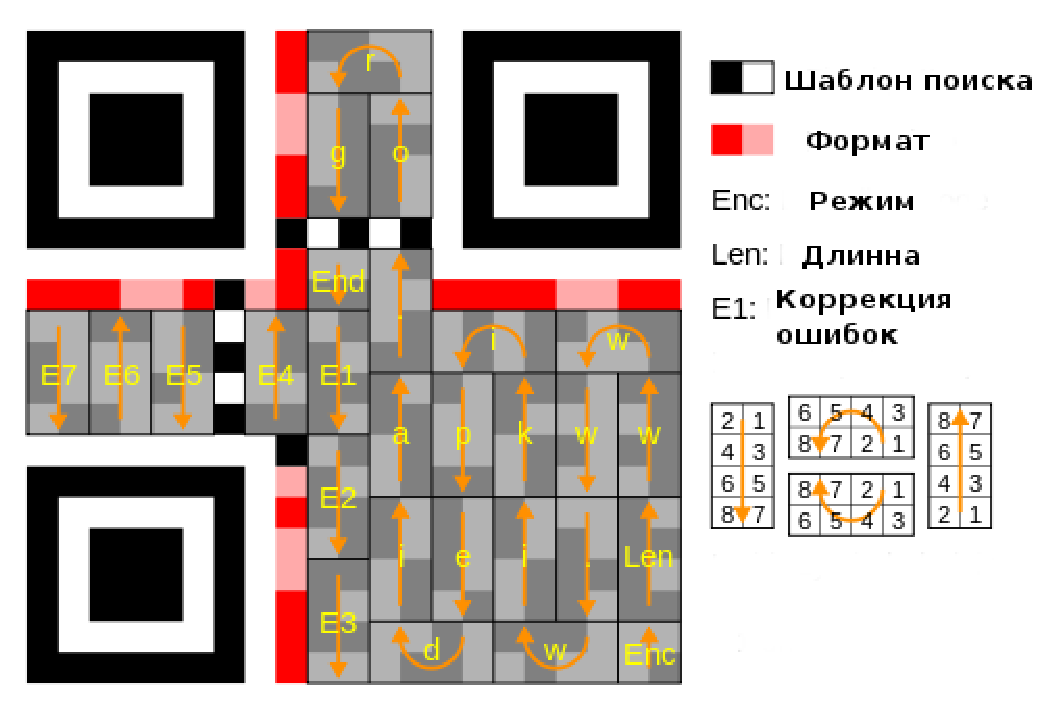
\includegraphics[scale=0.5]{img/qr_decode}
    \caption{Пример декодирования QR-кода}
    \label{fig:qrDecode}
\end{figure}


\subsubsection{Data Matrix}
Data Matrix --- двумерный штрихкод (описывается стандартом 
% ГОСТ Р ИСО/МЭК 16022--2008, аналогом ISO/IEC 16022:2006 \cite{bib:gostDM}),
позволяющий 
закодировать до 2335 алфавитно-цифровых символов, либо до 3116 цифр, 
либо до 1556 байтов информации (см. \figurename\ \ref{fig:dmSample}). 
Data Matrix, как и все другие подобные 
штрихкоды, содержит информацию для восстановления, которая позволяет 
восстановить закодированную информацию при частичном повреждении кода.

\begin{figure}[htb]
    \centering
    
\includegraphics{img/dm_sample}
    \caption{Штрихкод в формате Data Matrix}
    \label{fig:dmSample}
\end{figure}

Каждый код Data Matrix содержит две сплошные пересекающиеся линии в 
виде буквы L, для ориентации считывающего устройства, две другие 
границы кода состоят из перемежающихся чёрных и белых точек и служат для 
указания размеров кода считывающему устройству 
(см. \figurename\ \ref{fig:dmPattern}). Размер кода может быть от
$10 \times 10$ до $144 \times 144$ барселей (существую также 
прямоугольные версии для цилиндрических поверхностей). Дополнительно
можно объединять до 16 кодов в один большой символ.
На рисунке \ref{fig:dmCoding} показано,
как размещаются байты в штрихкоде.

\begin{figure}[htb]
    \centering
    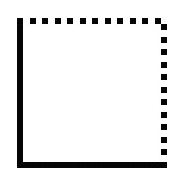
\includegraphics{img/dm_pattern}
    \caption{Шаблон поиска в штрихкоде Data Matrix}
    \label{fig:dmPattern}
\end{figure}

\begin{figure}[htb]
    \centering
    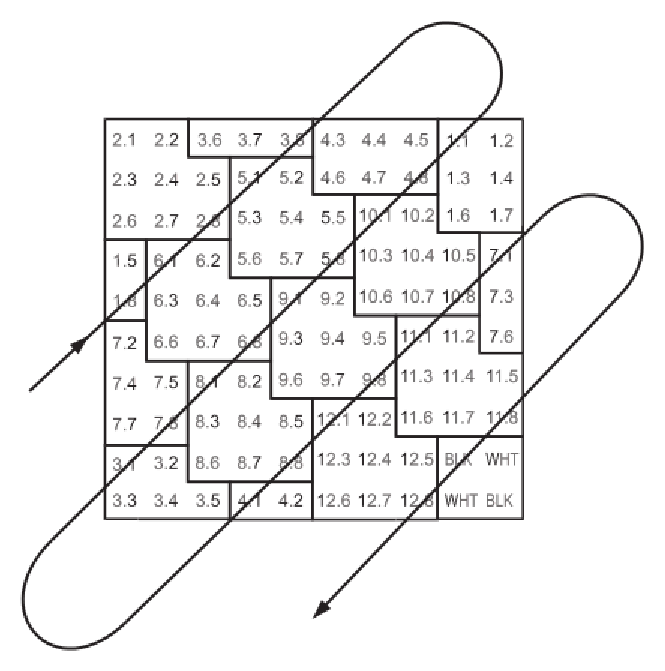
\includegraphics[scale=0.8]{img/dm_coding}
    \caption{Расположение байтов в Data Matrix}
    \label{fig:dmCoding}
\end{figure}

Все коды используют коррекцию ошибок стандарта ECC200, 
который, в свою очередь, использует алгоритм Рида-Соломона для 
кодирования/декодирования данных. Это позволяет восстановить в случае 
повреждения кода до 30\% полезной информации.

В промышленности Data Matrix применяют для маркировки различных элементов. 
Код может быть нанесён различными способами --- струйной печатью, гравировкой, 
лазером, электролитическими способами и т.д. В зависимости от метода нанесения, 
код может оставаться на элементе на протяжении всего его цикла 
использования (\figurename\ \ref{fig:dmSample2}).

\begin{figure}[htb]
    \centering
    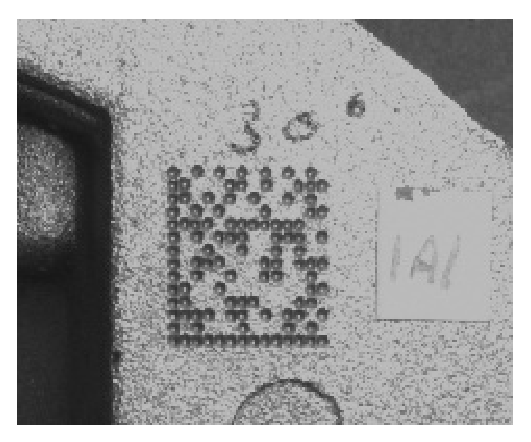
\includegraphics[scale=0.7]{img/dm_sample2}
    \caption{Штрихкод Data Matrix нанесённый методом иглографии}
    \label{fig:dmSample2}
\end{figure}

Основным положительным отличием Data Matrix от остальных двухмерных штрихкодов 
является то, что Data Matrix работает максимально быстро и небольшие объёмы 
данных осуществляются на минимальных площадях. Так, если кодировать 6 цифр, 
Data Matrix составит штрих-код размером $10 \times 10$ модулей, 
а вот если кодировать 
в Aztec, то эта площадь будет составлять $15 \times 15$ модулей. 
Но в то же время, 
данное преимущество теряется в процессе кодирования большего объёма информации: 
при одинаковых размерах символа в $132 \times 132$ модуля, Aztec закодирует  
почти 3000 
цифр, а Data Matrix максимум 2608. И при кодировании буквенно-цифровых данных 
в 10 символов, штрих-код Data Matrix занимает одинаковую площадь с Aztec. Чем 
же объясняется столь успешное кодирование малых пользовательских данных? Прежде 
всего, малым количеством служебной информации в составляемом коде, экономия 
производится за счёт размеров и структуры данных штрих-кода, таким образом 
надёжность считывания несколько падает. Также, Data Matrix имеет ещё один 
недостаток --- рост размера шаблона поиска символов увеличивается прямо 
пропорционально самому периметру символа, таким образом, становится невыгодным 
кодирование больших объёмов данных, у Aztec же шаблон поиска не изменяется.

\begin{table}[htb]
\centering
\caption{Таблица возможностей Data Matrix}
\begin{tabular}{|c|c|c|c|}
    \hline 
    Размер & \multicolumn{3}{c|}{Количество кодируемой информации} \\ 
    
    \hline 
    Ширина $\times$ Высота & Шифры & Символы & Байты \\
    
    \hline 
    $10 \times 10$ & 6 & 3 & 1 \\
    
    \hline 
    $12 \times 12$ & 10 & 6 & 3 \\
    
    \hline 
    $14 \times 14$ & 16 & 10 & 6 \\
    
    \hline 
    $16 \times 16$ & 24 & 16 & 10 \\
    
    \hline 
    $18 \times 18$ & 36 & 25 & 16 \\
    
    \hline 
    $20 \times 20$ & 44 & 31 & 20 \\
    
    \hline 
    $22 \times 22$ & 60 & 43 & 28 \\
    
    \hline 
    $24 \times 24$ & 72 & 52 & 34 \\
    
    \hline 
    $26 \times 26$ & 88 & 64 & 42 \\
    
    \hline 
    $32 \times 32$ & 124 & 91 & 60 \\
    
    \hline 
    $40 \times 40$ & 228 & 169 & 112 \\
    
    \hline 
    $44 \times 44$ & 288 & 214 & 142 \\
    
    \hline 
    $48 \times 48$ & 348 & 259 & 172 \\
    
    \hline 
    $52 \times 52$ & 408 & 304 & 202 \\
    
    \hline 
    $64 \times 64$ & 560 & 418 & 278 \\
    
    \hline 
    $72 \times 72$ & 736 & 550 & 366 \\
    
    \hline 
    $80 \times 80$ & 912 & 682 & 454 \\
    
    \hline 
    $88 \times 88$ & 1152 & 862 & 574 \\
    
    \hline 
    $96 \times 96$ & 1392 & 1042 & 694 \\
    
    \hline 
    $104 \times 104$ & 1632 & 1222 & 814 \\
    
    \hline 
    $120 \times 120$ & 2100 & 1573 & 1048 \\
    
    \hline 
    $132 \times 132$ & 2608 & 1954 & 1302 \\
    
    \hline 
    $144 \times 144$ & 3116 & 2335 & 1556 \\    
     
    \hline 
    \hline
    $8 \times 18$ & 10 & 6 & 3 \\
    
    \hline
    $8 \times 32$ & 20 & 13 & 8 \\
    
    \hline
    $12 \times 26$ & 32 & 22 & 14 \\
    
    \hline
    $12 \times 36$ & 44 & 31 & 20 \\
    
    \hline
    $16 \times 36$ & 64 & 46 & 30 \\
    
    \hline
    $16 \times 48$ & 98 & 72 & 47 \\
    
    \hline
\end{tabular} 
\end{table}
 

\subsubsection{Aztec Code}

Aztec Code представляет собой универсальную символику двухмерного
штрихового кода. Как показано на рисунках \ref{fig:acSmall} и \ref{fig:acBig},
код представляет собой квадрат, 
содержащий матрицу квадратных элементов, в центре которой располагается 
<<мишень>> (<<bullseye\footnote{Т.е. <<бычий глаз>> }>>), 
составленная из концентрических квадратов. Aztec 
позволяет эффективно кодировать как малые, так и большие объемы данных 
(цифры --- до 3832, текст --- до 3067 или байты --- до 1914) с 
использованием высокоэффективного метода Рида-Соломона коррекции ошибок 
(см. \ref{sec:RSCode}). Код Aztec разработан специалистами фирмы 
HandHeld Products (Andy Longacre и Rob Hussey) и защищен патентом, но частично 
выпущен для общего использования. Международная Спецификация Символики для 
кода Aztec утверждена AIM USA в формате ISO и доступна через филиалы AIM.



\begin{figure}[htb]
    \begin{multicols}{2}
 
        \begin{center}
             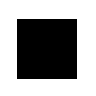
\includegraphics[]{img/ac_small} 
             \caption{<<Компактный>> символ Axtec Code}
             \label{fig:acSmall}
        \end{center}
   
        \begin{center}
            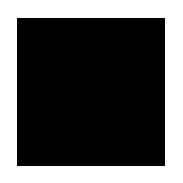
\includegraphics[]{img/ac_big} 
            \caption{<<Полноразмерный>> символ Axtec Code}
            \label{fig:acBig}
        \end{center}       
       
    \end{multicols}
\end{figure}

Квадратная <<мишень>>, окружённая <<слоями данных>>, сплетенными с решеткой 
<<элементов привязк>>, расположенной по периметру квадрата, дают в результате 
изображения ассоциирующееся с искусством Центральной Америки, что и подсказало 
имя <<Aztec Code>> для символики. 

Основные изменения в структуре кода и коррекции ошибок появились в Версии 2.0 
спецификации в июне 1995 года, но основная конструкция кода осталась 
неизменной, выдержав процесс отладки считывающих устройств, пробные внедрения 
и даже критический анализ, проведённый Техническим Комитетом (Technical 
Symbology Committee) AIM USA без изменений. Международная спецификация 
Aztec Code опубликована AIM International в 1997 году.

Существуют два основных формата символа Aztec Code: <<Compact>> (Компактный) 
символ с мишенью из двух квадратов (\figurename\ \ref{fig:acSmall}) и 
<<Full-Range>> (Полный) символ с мишенью из трёх квадратов 
(\figurename\ \ref{fig:acBig}). Поскольку принтеры могут автоматически 
выбирать, а сканеры автоматически распознавать оба формата, вместе два формата 
образуют последовательность из символов 33 различных размеров, которые могут 
эффективно кодировать как малые, так и большие сообщения. В общем, 
символы Aztec Code:

\begin{enumerate}
\item могут кодировать любую байтовую последовательность в эффективных 
компактных режимах для текстовых и цифровых данных;

\item всегда квадратной формы, изменяясь в размерах от $15 \times 15$ 
модулей до $151 \times 151$ модулей. Свободной зоны вокруг символа не 
требуется вообще. Таблица \ref{tableAc} показывает информационную ёмкость 
некоторых размеров кода;

\item может быть использован в структурном объединении, соединяющем 
до 26 символов;

\item имеет специальный формат настройки сканера, удобный для 
настройки сканера с помощью штрихкода. 
 
\end{enumerate}

\begin{table}[htb]
%TODO Make it as text
\centering
\caption{Соотношения размеров символов и ёмкости Aztec Code}
\label{tableAc}
\end{table}

Вид символа Aztec Code очень систематичен с чётко разграниченными 
функциями частей, обеспечивает простоту процедур кодирования и 
декодирования, в то же время его математическая структура необычайно 
гибка и надёжна.

Рисунок \ref{fig:acStruct} показывает структуру полного символа 
Aztec Code. Вы можете увидеть три постоянных элемента:

\begin{enumerate}
\item центральный указатель <<мишень>>;

\item элементы ориентации по углам указателя;

\item решётка привязки, пронизывающая область данных.

\end{enumerate} 

\begin{figure}[htb]
    \centering
    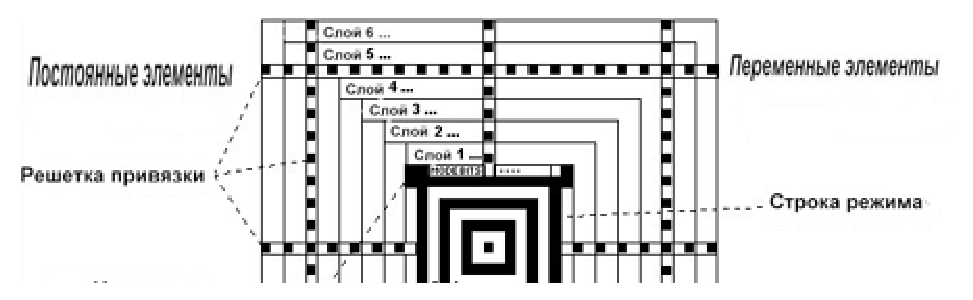
\includegraphics[scale=0.8]{img/ac_struct}
    \caption{Структура Aztec Code}
    \label{fig:acStruct}
\end{figure}
 
Два переменных элемента структуры\footnote{
Компактный символ Aztec Code содержит маленькую мишень без 
решётки привязки и только 4 слоя данных.} 
\begin{enumerate}
\item строка короткого режима, обернутая вокруг <<мишени>>;

\item от одного до 32 слоев данных толщиной в 2 барселя, 
спиралью расходящихся от центра.
\end{enumerate}

Строка короткого режима и слои данных закодированы с защитой от ошибок по 
методу Рида-Соломона. Строка режима --- это строка фиксированной длины, 
которая просто кодирует два параметра, несущие информацию о слоях данных, 
а именно: сколько слоев данных содержит данный символ и сколько слов 
содержится в сообщении (остаток места в области данных заполняется 
контрольными словами). Таким образом, уровень коррекции ошибок в Aztec Code 
становится регулируемым по указанию пользователя, и в принципе, слои 
данных могут содержать от 5\% до 95 \% контрольных слов, но на практике 
обычно нецелесообразно изменять стандартное значение в 23\% контрольных слов.

Слои данных, конечно, содержат последовательность кодовых слов, которые 
сперва кодируют пользовательские данные, затем добавляют к ним выявление и 
коррекцию ошибок. Защита от ошибок, кроме того, регулируемая пользователем 
и использующая дополнительные контрольные слова для заполнения, дополнительно 
усилена двумя путями: во-первых, размер кодового слова зависит от размера 
символа, от 6 бит для наименьших символов до 12 бит для наибольших, исключая 
необходимость чередующихся полей и обеспечивая хорошую зернистость для всех 
размеров символов. Во-вторых, слова сообщения, занимающие внешние слои символа, 
поддерживают чистовую коррекцию ошибок в стёртых углах символа.

В результате представленного рассмотрения технологии становятся понятными 
некоторые особенности Aztec Code: 

\begin{enumerate}
\item Слоёная природа полей данных обеспечивает целостность символов 33 
различных размеров и информационной ёмкости.

\item Указатель в виде мишени обеспечивает считывание при большом изменении 
угла сканирования.

\item Элементы ориентации дают возможность считывания при любой ориентации 
символа, включая зеркальное отражение. 

\item Решётка привязки позволяет учитывать существенные искривления 
больших символов.

\item Декодирование от центра к краю исключает необходимость полей 
(свободной зоны) вокруг символа.

\item Надёжный управляемый пользователем механизм коррекции ошибок по 
методу Рида-Соломона обеспечивает высокую производительность и надёжную 
защиту от ошибок. 

\item Расположение полей, устойчивых к появлению ошибок и повреждений, 
по краям символа, компенсирует влияние оптических искажений, возникающих 
по краям зоны сканирования.

\end{enumerate}

Aztec Code представляет собой универсальную символику 
матричного штрихового кода, хорошо приспособленную для визуальной технологии 
считывания и для кодирования как малых, так и больших объёмов данных. 
Aztec Code интересен для применений, требующих размещения кода на ограниченном 
пространстве (производство, коммерция, медицина, фармацевтика и т.д.), 
поскольку код обеспечивает высокую плотность размещения информации и не 
требует свободного пространства вокруг кода. Некоторые почтовые ведомства 
рассматривают возможность использования Aztec Code в качестве <<электронного 
штампа>> почтового отправления, в то же время электронное кодирование подписи 
с помощью Aztec привлекло внимание некоторых транспортных компаний.

\subsection{\textsc{Эффективность кода}}

\textit{Эффективностью штрихкода} $C$ назовём величину 

\begin{equation}
	\label{eq:theta}
	\theta_C(b, q) = \frac{b}{d(b, q)},
\end{equation}
где $d(b, q)$ ---
число барселей, которые необходимы для того, чтобы зашифровать сообщение
длинной $b$ бит при конфигурации кода $q$ (отражает 
уровень коррекции ошибок и т.д.). 

Другими словами, эффективность кода отражает число бит полезной
информации которое несёт в себе каждый барсель рассматриваемого 
кода $C$.

\textit{Предельной эффективностью кода} назовём величину

\begin{equation}
	\label{eq:Theta}
	\Theta_C(q) = \lim_{b \to \infty }\theta_C(b, q).
\end{equation}

Для рассмотренных выше кодов имеет место (принимаем во внимание,
что коды чёрно-белые, а значит один барсель~--- один бит):

\begin{equation*}
    d(b, q) = b + 2 \lceil b g(q) \rceil + f(b, q) + s (b, q),
\end{equation*}
где $g(q)$ --- текущий уровень коррекции ошибок (везде используется 
коды Рида-Соломона, поэтому на исправление одной ошибки требуется два 
дополнительных символа (см. \ref{sec:RSCode})), $f(b, q)$ --- свободное
место в матрице,  $s (b, q)$ --- служебная информация в коде\footnote{
В случае, когда каждый барсель может находиться в более чем двух состояниях
$k$ будем иметь:
\begin{equation*}
    d(b, q) = \frac{b+ 2 \lceil b g(q) \rceil}{\log_2 k}  + f(b, q) + s (b, q),
\end{equation*}
}. 
Принимая
во внимание тот факт, что $f(b, q) = o(b)$, a также $f(b, q) = o(b)$
(действительно, в рассматриваемых кодах информация записывается таким 
образом, что свободное место минимизируется; а служебные данные с возрастанием 
информации практически не возрастают) имеем\footnote{
Соответственно, для случая, описанного в предыдущем примечании:
\begin{equation}
	\Theta_C(q) = 
	    \frac{\log_2 k}{1 + 2g(q)}.
\end{equation}
}

\begin{equation}
	\Theta_C(q) = \lim_{b \to \infty } \frac
	    {b}
	    {b +2 \lceil b g(q) \rceil + o(b)} = 
	    \frac{1}{1 + 2g(q)}.
\end{equation}